\scanpage{16}
\diagram{\begin{tikzcd}Z\arrow[r,"\varphi"]\arrow[dr,"\deleted{\varphi}h"']&X\arrow[d,"f",no head]&Y\arrow[dl,"g",no head]\\&S&\end{tikzcd}}
\diagram{\begin{tikzcd}Z'\arrow[r,"\varphi'"]\arrow[rr,bend left=25,"v"]\arrow[dr,"h'"']&X'\arrow[r,"u"']\arrow[d,"f'"]&Y'\arrow[dl,"g'"]\\&S'&\end{tikzcd}}
\margin{Énoncer plutôt en termes de $\prod_{X/S}P/X\longrightarrow\prod_{Z/S}\unsure{Q}/Z$}
\figure{\begin{tikzpicture}[x=1cm,y=1cm]\draw (0,0)--(5.1,0);\draw (2.4,0)--(2.44,1.8);\draw(.95,-.18)--(.96,-.7);\end{tikzpicture}}

$f,h$ plat et propre sur $S$ loc. noeth

$g$ \deleted{\unsure{séparé}} de type fini [et séparé !]
\margin{\figure{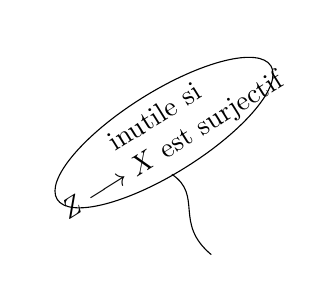
\begin{tikzpicture}\node[rotate=32,align=center] at(0,0){inutile si\\$Z\longrightarrow X$ est \uline{surjectif}};\draw[rotate=32](0,0)ellipse(1.6 and .52);\draw(.1,-.53)..controls(.5,-.8)and(.12,-1.15)..(.6,-1.55);\end{tikzpicture}}}
\margin{\uline{N.B.} l'hypothèse $S$ loc. noeth peut être remplacée par des hypothèses de présentation finie sur $f,g,h$.}
\unsure{a un mor}
\diagram{\begin{tikzcd}[cells={nodes={draw=gray,ellipse,inner xsep=8pt,inner ysep=5pt}},column sep=large]\underline{\operatorname{Hom}}_S(X,Y)\arrow[r]&\underline{\operatorname{Hom}}_S(Z,Y)\end{tikzcd}}
Pour $\varphi$\ldots

a) Le sous-foncteur de $\underline{\operatorname{Hom}}_S(X,Y)$ où $\underline{\operatorname{Hom}}_S(X,Y)$ est non \uline{ramifié} sur $\unsure{\varphi}$ \inserted{$\underline{\operatorname{Hom}}(Z,Y)$}, est un sous-foncteur ouvert.

Il correspond à $u':X'\longrightarrow Y'$ tel que, pour tout $s\in S'$,
\[
\operatorname{Hom}(u_s^{\unsure{\prime|\circ}*}(\Omega^1_{Y'_s/k(s)}),k(s))-\operatorname{Hom}(v_s^{\unsure{\prime|\circ}*}(\Omega^1_{Y'_s/k(s)}),k(s))
\]
est injectif. \uline{Or} on peut trouver sur $S'$ des Modules \uline{cohérents} $M_u,M_v$ tels que pour tt $J$ qu. coh. sur $S'$, on ait des isom \unsure{fonctoriels|naturels}
\[
\operatorname{Hom}_{\underline{O}_{X'}}(u^*(\Omega^1_{Y'/S'}),\unsure{\underline{O}_{X'}|f_{X'}}\otimes_{\underline{O}_{S'}}J)\simeq\operatorname{Hom}_{\underline{O}_{\unsure{S|S'}}}(M_u,J)
\]
\[
\operatorname{Hom}_{\underline{O}_{Z'}}(v^*\Omega^1_{Y'/S'},\underline{O}_{Z'}\otimes_{\underline{O}_{S'}}J)\simeq\operatorname{Hom}_{\underline{O}_{\unsure{S|S'}}}(M_v,J)
\]
\margin{N.B. \uline{\unsure{réduction}} \uline{immédiate} \uline{au cas} $S'$ \uline{artinien}}
et la formation de $M_u,M_v$ est compatible avec l'extension de la base. Ceci dit, on a un hom naturel
\[
(*)\qquad M_v\longrightarrow M_u
\]
qui définit par $\operatorname{Hom}(\ ,J)$ l'hom naturel
\[
\operatorname{Hom}_{\underline{O}_{X'}}(u^*\Omega^1_{Y'/S'},\underline{O}_{X'}\otimes_{\underline{O}_{S'}}J)\longrightarrow\operatorname{Hom}_{\underline{O}_{Z'}}(v^*\Omega^1_{Y'/S'},\underline{O}_{Z'}\otimes_{\underline{O}_{S'}}J).
\]
Dire \deleted{Alors} \inserted{que} la condition de non ramification est satisfaite en un pt $s\in S'$, signifie qu'en ce point
\[
M_v\otimes k(s)\longrightarrow M_u\otimes k(s)
\]
est \uline{surjectif}, et par Nakayama ceci restera vrai en
\mspage{15}
